\documentclass[11pt]{article}
\usepackage{graphicx}
\usepackage{hyperref}
\usepackage{appendix}
\usepackage{amsmath}
\usepackage{amsthm}
\usepackage{amssymb}
\usepackage{float}
\usepackage{multirow}
\usepackage{commath}
\usepackage{booktabs}
\renewcommand{\arraystretch}{1.2}
\usepackage{siunitx}
\sisetup{detect-all}
\usepackage{listings}
\usepackage{color} %red, green, blue, yellow, cyan, magenta, black, white
\definecolor{mygreen}{RGB}{28,172,0} % color values Red, Green, Blue
\definecolor{mylilas}{RGB}{170,55,241}
\usepackage[a4paper,margin=20mm]{geometry}
\numberwithin{equation}{section}
\setlength{\parskip}{\baselineskip}
\setlength{\parindent}{0pt}
\hypersetup{
    colorlinks=true,
    linkcolor=black,
    filecolor=black,      
    urlcolor=black,
    citecolor=black
}
\urlstyle{same}
\begin{document}
\title{\textbf{UCL Mechanical Engineering 2020/2021}\\MECH0011 Final Coursework}
\author{NCWT3}
\maketitle
\tableofcontents
\listoffigures
\section{Question 1}
\subsection{a}
The data was imported into MATLAB and the shape of the hydrofoil, the chord line and the mean camber line were plotted for all four hydrofoils.
\lstset{language=Matlab,%
    %basicstyle=\color{red},
    breaklines=true,%
    morekeywords={matlab2tikz},
    keywordstyle=\color{blue},%
    morekeywords=[2]{1}, keywordstyle=[2]{\color{black}},
    identifierstyle=\color{black},%
    stringstyle=\color{mylilas},
    commentstyle=\color{mygreen},%
    showstringspaces=false,%without this there will be a symbol in the places where there is a space
    numbers=left,%
    numberstyle={\tiny \color{black}},% size of the numbers
    numbersep=9pt, % this defines how far the numbers are from the text
    emph=[1]{for,end,break},emphstyle=[1]\color{red}, %some words to emphasise
    %emph=[2]{word1,word2}, emphstyle=[2]{style},    
}
\lstinputlisting{./mCode/q1a.m}
\begin{figure}[H]
    \centering
    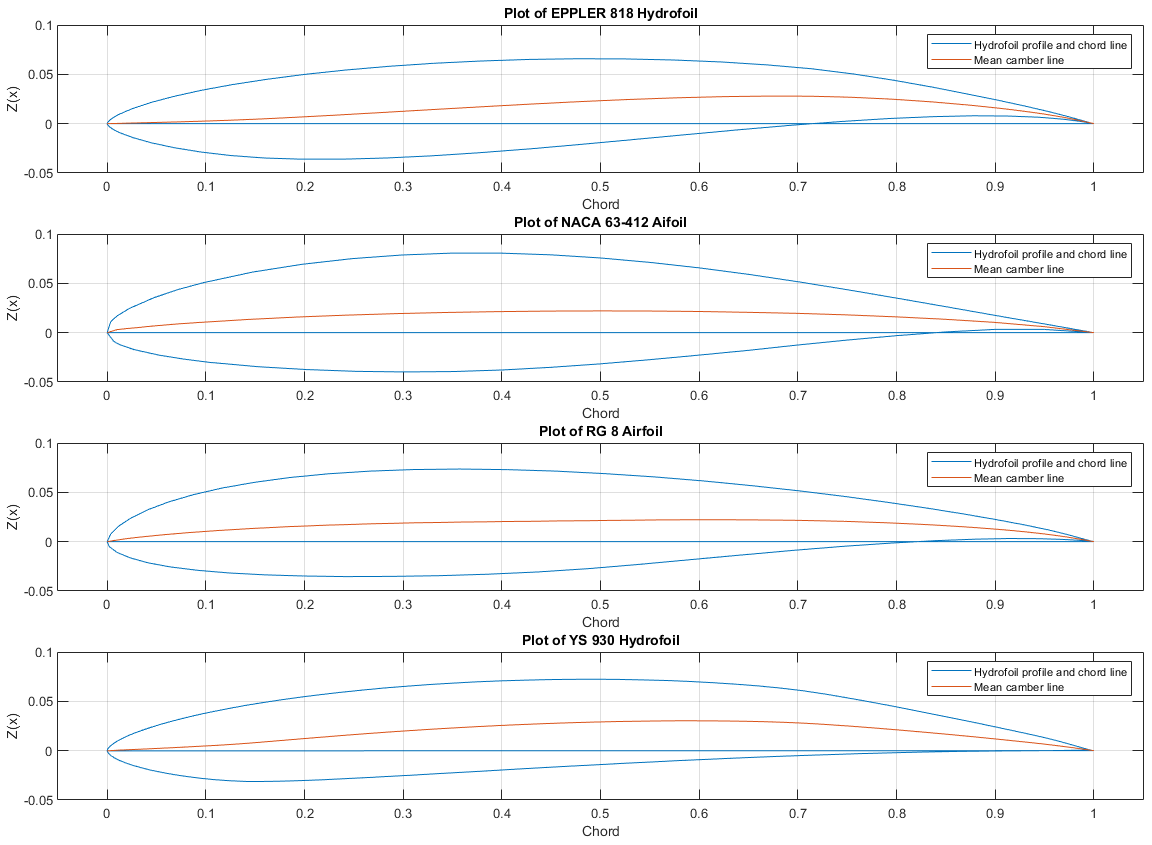
\includegraphics[width = \textwidth]{./img/q1a.png}
    \caption{Graphs to show hydrofoil shape, chord line and mean camber line for four different hydrofoils.}
    \label{fig:q1a}
\end{figure}
\subsection{b}
MATLAB was used to calculate the lift-to-drag ratio for each hydrofoil.
\lstset{language=Matlab,%
    %basicstyle=\color{red},
    breaklines=true,%
    morekeywords={matlab2tikz},
    keywordstyle=\color{blue},%
    morekeywords=[2]{1}, keywordstyle=[2]{\color{black}},
    identifierstyle=\color{black},%
    stringstyle=\color{mylilas},
    commentstyle=\color{mygreen},%
    showstringspaces=false,%without this there will be a symbol in the places where there is a space
    numbers=left,%
    numberstyle={\tiny \color{black}},% size of the numbers
    numbersep=9pt, % this defines how far the numbers are from the text
    emph=[1]{for,end,break},emphstyle=[1]\color{red}, %some words to emphasise
    %emph=[2]{word1,word2}, emphstyle=[2]{style},    
}
\lstinputlisting{./mCode/q1b.m}
\begin{figure}[H]
    \centering
    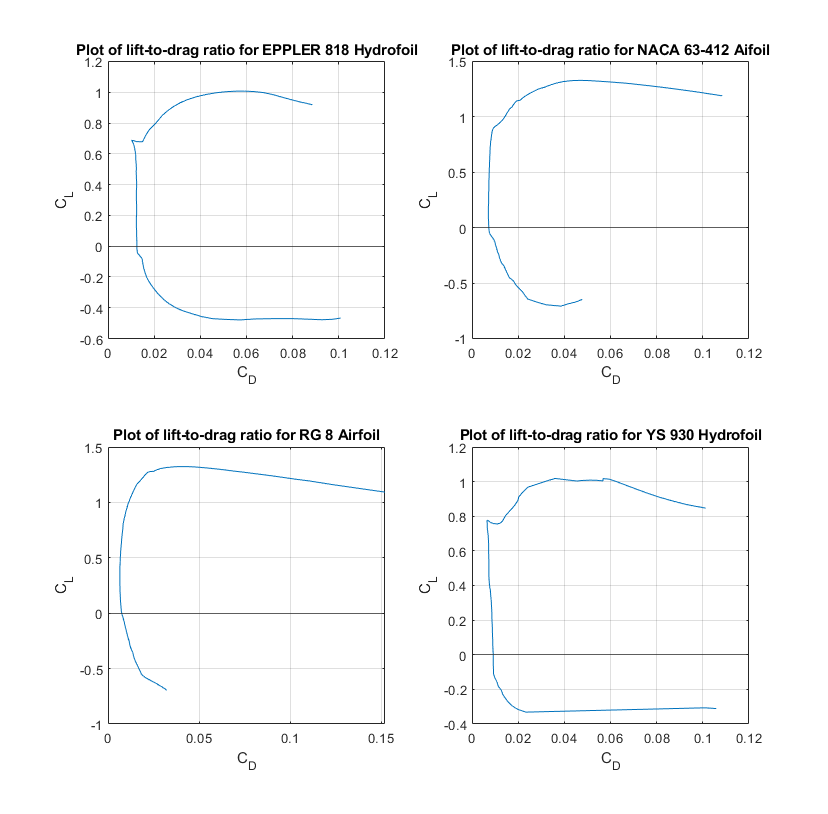
\includegraphics[height = 10cm]{./img/q1b.png}
    \caption{Graph to show lift-to-drag ratio for four different hydrofoils.}
    \label{fig:q1b}
\end{figure}
\subsection{c}
At a low angle of attack, the flow is attached to the hydrofoil and separates close to the trailing edge, leaving a small wake. The streamlined shape of the hydrofoil exerts a large shear force on the flow passing over it, leading to a large skin drag but low form drag. As we increase the angle of attack, the flow separation moves along the top of the hydrofoil. This decreases the shear force acting on the hydrofoil and the skin drag starts to reduce, with form drag increasing. At the stall angle, the pressure distribution along the top of the hydrofoil dramatically changes due to flow separation, suction pressure is mostly/all lost and a large wake with turbulent effects is present. The primary drag effect here is now form drag, as the flow is not attached along the length of the hydrofoil surface.
\subsection{d}
MATLAB was used to calculate each of the variables for each hydrofoil.
\lstset{language=Matlab,%
    %basicstyle=\color{red},
    breaklines=true,%
    morekeywords={matlab2tikz},
    keywordstyle=\color{blue},%
    morekeywords=[2]{1}, keywordstyle=[2]{\color{black}},
    identifierstyle=\color{black},%
    stringstyle=\color{mylilas},
    commentstyle=\color{mygreen},%
    showstringspaces=false,%without this there will be a symbol in the places where there is a space
    numbers=left,%
    numberstyle={\tiny \color{black}},% size of the numbers
    numbersep=9pt, % this defines how far the numbers are from the text
    emph=[1]{for,end,break},emphstyle=[1]\color{red}, %some words to emphasise
    %emph=[2]{word1,word2}, emphstyle=[2]{style},    
}
\lstinputlisting{./mCode/q1d.m}
\begin{table}[H]
    \centering
    \begin{tabular}{@{}llll@{}}
    \toprule
        & \multicolumn{3}{c}{Maximum}\\
        \cline{2-4}
        Hydrofoil& \% camber & \% thickness & lift coefficient \\
    \midrule
        EPPLER 818 Hydrofoil & 2.792 & 9.362  & 1.008 \\
        NACA 63-412 Aifoil   & 2.204 & 11.992 & 1.330 \\
        RG 8 Airfoil         & 2.226 & 10.795 & 1.323 \\
        YS 930 Hydrofoil     & 3.028 & 9.088  & 1.018 \\ 
    \bottomrule
    \end{tabular}
    \caption{Table to show maximum percentage camber and thickness and the maximum lift coefficient for four hydrofoils.}
\end{table}
\begin{table}[H]
    \centering
    \begin{tabular}{@{}llll@{}}
    \toprule
        & & Lift coefficient & Angle of attack $\alpha_0$\\
        Hydrofoil & Stall angle  & for $\alpha = \SI{0}{\degree}$ & corresponding to $C_L = 0$\\
    \midrule
        EPPLER 818 Hydrofoil & \SI{7.75}{\degree}  & 0.361 & \SI{-3}{\degree}    \\
        NACA 63-412 Aifoil   & \SI{13}{\degree}    & 0.338 & \SI{-3}{\degree}  \\
        RG 8 Airfoil         & \SI{12.75}{\degree} & 0.382 & \SI{-3}{\degree} \\
        YS 930 Hydrofoil     & \SI{9}{\degree}  & 0.391 & \SI{-3.75}{\degree}  \\ 
    \bottomrule
    \end{tabular}
    \caption{Table to show the stall angle, lift coefficient for $\alpha = \SI{0}{\degree}$ and the angle of attack $\alpha_0$ corresponding to $C_L = 0$ for four hydrofoils.}
\end{table}
The hydrofoils both have a higher percentage camber than the airfoils. They also have a lower percentage thickness than the airfoils. We can see that this leads to a reduction in the stall angle and subsequently their maximum lift coefficients are lower. However, we can see that they perform better at $\alpha = \SI{0}{\degree}$. This can be attributed to the fact that at small $\alpha$, larger camber generates more lift, at the expense of a smaller stall angle, as the boundary layer is more prone to separation at higher $\alpha$. However, increasing either percentage camber or thickness will increase $C_D$.
\subsection{e}
The RG 8 Airfoil was selected as it has a high stall angle, with a subsequently large maximum lift coefficient, the lift coefficient at $\alpha = \SI{0}{\degree}$ is also the second highest. We can calculate the lift on the hydrofoil using \ref{eq:q1e1}:
\begin{equation}
    L = \frac{1}{2}\rho C_L V_{w}^2 A \label{eq:q1e1}
\end{equation}
where $\rho$ is the density of seawater, $C_L$ is the lift coefficient for a given angle of attack, $V_w$ is the velocity of the fluid relative to the wing and $A$ is the projected surface area of the wing. The surface area $A$ can be found by integration:
\begin{align}
    A &= \int_{x_0}^{b + x_0} \left(-0.07x + c_0\right)\dif x\\
    A &= \left[-0.035x^2 + c_0x\right]_{x_o}^{b+x_0}
\end{align}
$x_0 = 0.1$ as given in the material. I have also selected $b = \SI{2}{\meter}$, hence:
\begin{align}
    A &= -0.035(2.1)^2 + c_0(2.1) + 0.035(0.1)^2 - c_0(0.1)\\
    A &= 2c_0 - 0.154 \label{eq:q1e2}
\end{align}
Substituting \ref{eq:q1e2} into \ref{eq:q1e1}:
\begin{align}
    L = \frac{1}{2}\rho C_L V_{w}^2 \left(2c_0 - 0.154\right)
\end{align}
Rearranging for $c_0$:
\begin{align}
    \left(2c_0 - 0.154\right) &= \dfrac{L}{\frac{1}{2}\rho C_L V_{w}^2}\\
    c_0 &= \dfrac{L}{\rho C_L V_{w}^2} + 0.077
\end{align}
The following values were used: $\rho = \SI{1036}{\kg\per\meter\cubed}$ \cite{b1}, $V_w = \SI{11}{\meter\per\second}$ (\SI{39.6}{\kilo\meter\per\hour}), $L = 2000\times 9.81 \approx \SI{20000}{\newton}$. MATLAB was used to plot the chord length against the angle of attack. As $V_w$ represents the upper speed limit of the boat, we want to select a low angle of attack, to reduce the amount of drag on the foil. Hence, the value for $C_L$ at $\alpha = 0$ will be used. 
\lstset{language=Matlab,%
    %basicstyle=\color{red},
    breaklines=true,%
    morekeywords={matlab2tikz},
    keywordstyle=\color{blue},%
    morekeywords=[2]{1}, keywordstyle=[2]{\color{black}},
    identifierstyle=\color{black},%
    stringstyle=\color{mylilas},
    commentstyle=\color{mygreen},%
    showstringspaces=false,%without this there will be a symbol in the places where there is a space
    numbers=left,%
    numberstyle={\tiny \color{black}},% size of the numbers
    numbersep=9pt, % this defines how far the numbers are from the text
    emph=[1]{for,end,break},emphstyle=[1]\color{red}, %some words to emphasise
    %emph=[2]{word1,word2}, emphstyle=[2]{style},    
}
\lstinputlisting{./mCode/q1e.m}
Our chord length is calculated to be $c_0 = \SI{0.4948}{\meter}$. We must now check whether this chord length is sufficient to lift the boat at lower speeds. In order to do this we require a high angle of attack, to generate more lift. The value for $C_L$ at \SI{11}{\degree} was used to test the lift at $\SI{6}{\meter\per\second}$ ($\SI{21.6}{\kilo\meter\per\hour}$) and MATLAB gives a lift value of \SI{20215}{\newton}, allowing the boat to be out of the water at lower speeds as well.
\section{Question 2}
\section{Question 3}
\subsection{a}
MATLAB was used to plot the boundary layer velocity profile.
\lstset{language=Matlab,%
    %basicstyle=\color{red},
    breaklines=true,%
    morekeywords={matlab2tikz},
    keywordstyle=\color{blue},%
    morekeywords=[2]{1}, keywordstyle=[2]{\color{black}},
    identifierstyle=\color{black},%
    stringstyle=\color{mylilas},
    commentstyle=\color{mygreen},%
    showstringspaces=false,%without this there will be a symbol in the places where there is a space
    numbers=left,%
    numberstyle={\tiny \color{black}},% size of the numbers
    numbersep=9pt, % this defines how far the numbers are from the text
    emph=[1]{for,end,break},emphstyle=[1]\color{red}, %some words to emphasise
    %emph=[2]{word1,word2}, emphstyle=[2]{style},    
}
\lstinputlisting{./mCode/q3a.m}
\begin{figure}[H]
    \centering
    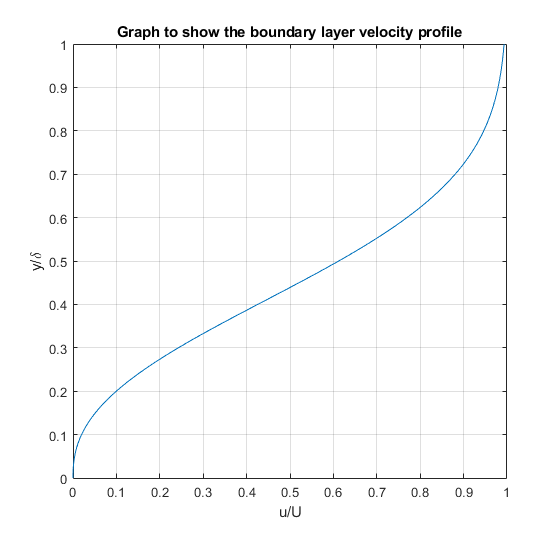
\includegraphics[height = 8cm]{./img/q3a.png}
    \caption{Graph to show boundary layer velocity profile.}
    \label{fig:q3a}
\end{figure}
\begin{thebibliography}{00}
    \bibitem{b1} Pawlowicz, R. (2013) Key Physical Variables in the Ocean: Temperature, Salinity, and Density. Nature Education Knowledge 4(4):13 \url{https://www.nature.com/scitable/knowledge/library/key-physical-variables-in-the-ocean-temperature-102805293/} Accessed: 19/05/2021 00:00
\end{thebibliography}
\end{document}